% Options for packages loaded elsewhere
\PassOptionsToPackage{unicode}{hyperref}
\PassOptionsToPackage{hyphens}{url}
\PassOptionsToPackage{dvipsnames,svgnames,x11names}{xcolor}
%
\documentclass[
  letterpaper,
  DIV=11,
  numbers=noendperiod]{scrartcl}

\usepackage{amsmath,amssymb}
\usepackage{iftex}
\ifPDFTeX
  \usepackage[T1]{fontenc}
  \usepackage[utf8]{inputenc}
  \usepackage{textcomp} % provide euro and other symbols
\else % if luatex or xetex
  \usepackage{unicode-math}
  \defaultfontfeatures{Scale=MatchLowercase}
  \defaultfontfeatures[\rmfamily]{Ligatures=TeX,Scale=1}
\fi
\usepackage{lmodern}
\ifPDFTeX\else  
    % xetex/luatex font selection
\fi
% Use upquote if available, for straight quotes in verbatim environments
\IfFileExists{upquote.sty}{\usepackage{upquote}}{}
\IfFileExists{microtype.sty}{% use microtype if available
  \usepackage[]{microtype}
  \UseMicrotypeSet[protrusion]{basicmath} % disable protrusion for tt fonts
}{}
\makeatletter
\@ifundefined{KOMAClassName}{% if non-KOMA class
  \IfFileExists{parskip.sty}{%
    \usepackage{parskip}
  }{% else
    \setlength{\parindent}{0pt}
    \setlength{\parskip}{6pt plus 2pt minus 1pt}}
}{% if KOMA class
  \KOMAoptions{parskip=half}}
\makeatother
\usepackage{xcolor}
\ifLuaTeX
  \usepackage{luacolor}
  \usepackage[soul]{lua-ul}
\else
  \usepackage{soul}
  
\fi
\setlength{\emergencystretch}{3em} % prevent overfull lines
\setcounter{secnumdepth}{-\maxdimen} % remove section numbering
% Make \paragraph and \subparagraph free-standing
\makeatletter
\ifx\paragraph\undefined\else
  \let\oldparagraph\paragraph
  \renewcommand{\paragraph}{
    \@ifstar
      \xxxParagraphStar
      \xxxParagraphNoStar
  }
  \newcommand{\xxxParagraphStar}[1]{\oldparagraph*{#1}\mbox{}}
  \newcommand{\xxxParagraphNoStar}[1]{\oldparagraph{#1}\mbox{}}
\fi
\ifx\subparagraph\undefined\else
  \let\oldsubparagraph\subparagraph
  \renewcommand{\subparagraph}{
    \@ifstar
      \xxxSubParagraphStar
      \xxxSubParagraphNoStar
  }
  \newcommand{\xxxSubParagraphStar}[1]{\oldsubparagraph*{#1}\mbox{}}
  \newcommand{\xxxSubParagraphNoStar}[1]{\oldsubparagraph{#1}\mbox{}}
\fi
\makeatother


\providecommand{\tightlist}{%
  \setlength{\itemsep}{0pt}\setlength{\parskip}{0pt}}\usepackage{longtable,booktabs,array}
\usepackage{calc} % for calculating minipage widths
% Correct order of tables after \paragraph or \subparagraph
\usepackage{etoolbox}
\makeatletter
\patchcmd\longtable{\par}{\if@noskipsec\mbox{}\fi\par}{}{}
\makeatother
% Allow footnotes in longtable head/foot
\IfFileExists{footnotehyper.sty}{\usepackage{footnotehyper}}{\usepackage{footnote}}
\makesavenoteenv{longtable}
\usepackage{graphicx}
\makeatletter
\def\maxwidth{\ifdim\Gin@nat@width>\linewidth\linewidth\else\Gin@nat@width\fi}
\def\maxheight{\ifdim\Gin@nat@height>\textheight\textheight\else\Gin@nat@height\fi}
\makeatother
% Scale images if necessary, so that they will not overflow the page
% margins by default, and it is still possible to overwrite the defaults
% using explicit options in \includegraphics[width, height, ...]{}
\setkeys{Gin}{width=\maxwidth,height=\maxheight,keepaspectratio}
% Set default figure placement to htbp
\makeatletter
\def\fps@figure{htbp}
\makeatother
% definitions for citeproc citations
\NewDocumentCommand\citeproctext{}{}
\NewDocumentCommand\citeproc{mm}{%
  \begingroup\def\citeproctext{#2}\cite{#1}\endgroup}
\makeatletter
 % allow citations to break across lines
 \let\@cite@ofmt\@firstofone
 % avoid brackets around text for \cite:
 \def\@biblabel#1{}
 \def\@cite#1#2{{#1\if@tempswa , #2\fi}}
\makeatother
\newlength{\cslhangindent}
\setlength{\cslhangindent}{1.5em}
\newlength{\csllabelwidth}
\setlength{\csllabelwidth}{3em}
\newenvironment{CSLReferences}[2] % #1 hanging-indent, #2 entry-spacing
 {\begin{list}{}{%
  \setlength{\itemindent}{0pt}
  \setlength{\leftmargin}{0pt}
  \setlength{\parsep}{0pt}
  % turn on hanging indent if param 1 is 1
  \ifodd #1
   \setlength{\leftmargin}{\cslhangindent}
   \setlength{\itemindent}{-1\cslhangindent}
  \fi
  % set entry spacing
  \setlength{\itemsep}{#2\baselineskip}}}
 {\end{list}}
\usepackage{calc}
\newcommand{\CSLBlock}[1]{\hfill\break\parbox[t]{\linewidth}{\strut\ignorespaces#1\strut}}
\newcommand{\CSLLeftMargin}[1]{\parbox[t]{\csllabelwidth}{\strut#1\strut}}
\newcommand{\CSLRightInline}[1]{\parbox[t]{\linewidth - \csllabelwidth}{\strut#1\strut}}
\newcommand{\CSLIndent}[1]{\hspace{\cslhangindent}#1}

\KOMAoption{captions}{tableheading}
\makeatletter
\@ifpackageloaded{tcolorbox}{}{\usepackage[skins,breakable]{tcolorbox}}
\@ifpackageloaded{fontawesome5}{}{\usepackage{fontawesome5}}
\definecolor{quarto-callout-color}{HTML}{909090}
\definecolor{quarto-callout-note-color}{HTML}{0758E5}
\definecolor{quarto-callout-important-color}{HTML}{CC1914}
\definecolor{quarto-callout-warning-color}{HTML}{EB9113}
\definecolor{quarto-callout-tip-color}{HTML}{00A047}
\definecolor{quarto-callout-caution-color}{HTML}{FC5300}
\definecolor{quarto-callout-color-frame}{HTML}{acacac}
\definecolor{quarto-callout-note-color-frame}{HTML}{4582ec}
\definecolor{quarto-callout-important-color-frame}{HTML}{d9534f}
\definecolor{quarto-callout-warning-color-frame}{HTML}{f0ad4e}
\definecolor{quarto-callout-tip-color-frame}{HTML}{02b875}
\definecolor{quarto-callout-caution-color-frame}{HTML}{fd7e14}
\makeatother
\makeatletter
\@ifpackageloaded{caption}{}{\usepackage{caption}}
\AtBeginDocument{%
\ifdefined\contentsname
  \renewcommand*\contentsname{Table of contents}
\else
  \newcommand\contentsname{Table of contents}
\fi
\ifdefined\listfigurename
  \renewcommand*\listfigurename{List of Figures}
\else
  \newcommand\listfigurename{List of Figures}
\fi
\ifdefined\listtablename
  \renewcommand*\listtablename{List of Tables}
\else
  \newcommand\listtablename{List of Tables}
\fi
\ifdefined\figurename
  \renewcommand*\figurename{Figure}
\else
  \newcommand\figurename{Figure}
\fi
\ifdefined\tablename
  \renewcommand*\tablename{Table}
\else
  \newcommand\tablename{Table}
\fi
}
\@ifpackageloaded{float}{}{\usepackage{float}}
\floatstyle{ruled}
\@ifundefined{c@chapter}{\newfloat{codelisting}{h}{lop}}{\newfloat{codelisting}{h}{lop}[chapter]}
\floatname{codelisting}{Listing}
\newcommand*\listoflistings{\listof{codelisting}{List of Listings}}
\makeatother
\makeatletter
\makeatother
\makeatletter
\@ifpackageloaded{caption}{}{\usepackage{caption}}
\@ifpackageloaded{subcaption}{}{\usepackage{subcaption}}
\makeatother

\ifLuaTeX
  \usepackage{selnolig}  % disable illegal ligatures
\fi
\usepackage{bookmark}

\IfFileExists{xurl.sty}{\usepackage{xurl}}{} % add URL line breaks if available
\urlstyle{same} % disable monospaced font for URLs
\hypersetup{
  pdftitle={Estás en la EI1039},
  pdfauthor={Carlos Granell},
  colorlinks=true,
  linkcolor={blue},
  filecolor={Maroon},
  citecolor={Blue},
  urlcolor={Blue},
  pdfcreator={LaTeX via pandoc}}


\title{Estás en la EI1039}
\author{Carlos Granell}
\date{Sep 16, 2024}

\begin{document}
\maketitle


\subsection{Objetivo y resultados de
aprendizaje}\label{objetivo-y-resultados-de-aprendizaje}

Según el
\href{https://ujiapps.uji.es/sia/rest/publicacion/2025/estudio/225/asignatura/EI1039}{SIA},

\begin{quote}
``la asignatura Diseño de Software se imparte en el primer semestre de
cuarto curso del grado en Ingeniería Informática de la Universitat Jaume
I, como parte del itinerario de Ingeniería del Software. El objetivo de
esta asignatura es proporcionar al alumnado conocimientos y habilidades
sobre las distintas etapas del diseño del software dentro del proceso de
desarrollo.''
\end{quote}

Y al finalizar satisfactoriamente la EI1039, deberías ser capaz de:

\begin{itemize}
\tightlist
\item
  Comparar las distintas estrategias que se pueden utilizar en el diseño
  de un sistema software.
\item
  Seleccionar, aplicar y evaluar patrones de arquitectura y diseño
  adecuados a la resolución de un determinado problema de desarrollo del
  software.
\item
  Diseñar y evaluar la interfaz de usuario utilizando principios y
  técnicas propias de la interacción persona-computador.
\end{itemize}

Tan importantes, o incluso más, que los resultados de aprendizaje
mencionados anteriormente son las competencias blandas o habilidades
interpersonales (\emph{soft skills}), como la comunicación, el trabajo
en equipo, la síntesis de información, la toma de decisiones, la
resolución de conflictos, la gestión del tiempo, y el liderazgo.
Trabajaremos en estas competencias o habilidades a lo largo del curso
porque, aunque parezca increíble, son aspectos vitales del día a día de
un arquitecto/a o diseñador/a de software.

Arquitectura software, patrones de diseño, comunicación, trabajo en
equipo, \ldots. Suena bien, ¿no? Espero que encuentres atractivo e
interesante el contenido de la asignatura a lo largo del semestre.

\subsection{Método de instrucción}\label{muxe9todo-de-instrucciuxf3n}

\begin{tcolorbox}[enhanced jigsaw, left=2mm, colframe=quarto-callout-tip-color-frame, toprule=.15mm, rightrule=.15mm, toptitle=1mm, bottomtitle=1mm, breakable, opacityback=0, title=\textcolor{quarto-callout-tip-color}{\faLightbulb}\hspace{0.5em}{¿Te has preguntado alguna vez qué pasa en tu cerebro cuando aprendes?
{[}@lang2016{]}}, bottomrule=.15mm, coltitle=black, colback=white, titlerule=0mm, arc=.35mm, leftrule=.75mm, opacitybacktitle=0.6, colbacktitle=quarto-callout-tip-color!10!white]

Tenemos millones de neuronas que ``hacen amigos fácilmente''. Las
neuronas se conectan con otras neuronas con cada nueva experiencia que
tenemos (nuevas emociones, pensamientos, acciones, conocimiento, etc.)
formando redes. Las redes al principio son débiles, pero cada vez que
repetimos la experiencia o acción, es camimo de la red se consolida y se
hace más fuerte. \textbf{Cuando aprendemos, nuestro cerebro cambia} por
la formación de nuevas conexiones entre neuronas.

\end{tcolorbox}

\begin{tcolorbox}[enhanced jigsaw, left=2mm, colframe=quarto-callout-tip-color-frame, toprule=.15mm, rightrule=.15mm, toptitle=1mm, bottomtitle=1mm, breakable, opacityback=0, title=\textcolor{quarto-callout-tip-color}{\faLightbulb}\hspace{0.5em}{Pirámide Bloom}, bottomrule=.15mm, coltitle=black, colback=white, titlerule=0mm, arc=.35mm, leftrule=.75mm, opacitybacktitle=0.6, colbacktitle=quarto-callout-tip-color!10!white]

Cuando \textbf{reflexionamos} y \textbf{aplicamos} (en contraposición a
simplemente leer o subrayar, ver Figure~\ref{fig-bloom}) cierto
conocimiento a contextos nuevos, lo comprendemos más profundamente,
provocando que la red sea más densa y tenga conexiones con otras redes.
La differencia entre la red de un principiante y la de un experto radica
justamente en el número y densidad de conexiones\textbf{. Cuanto más
interconexiones, mayor comprensión}.

\begin{figure}[H]

\centering{

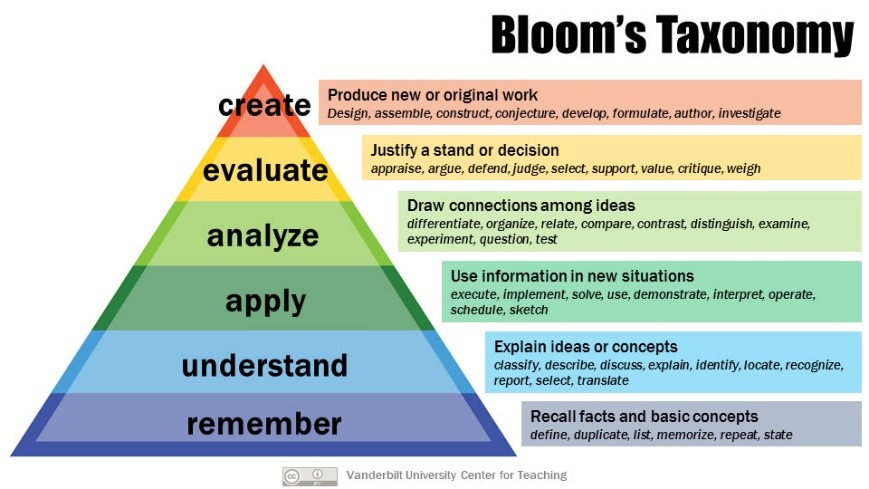
\includegraphics[width=3.64583in,height=\textheight]{images/bloom_taxonomy.jpg}

}

\caption{\label{fig-bloom}Taxonomía de Bloom}

\end{figure}%

\end{tcolorbox}

Si esperas presentaciones largas y densas por mi parte todos los viernes
por la tarde, entonces creo que te has matriculado de la asignatura
equivocada. 😁🍻

Hay evidencia científica de sobra que demuestra una y otra vez que los
métodos de \emph{aprendizaje activo} (por \emph{activo} me refiero a
todos, tanto dentro como fuera de clase) son mucho más efectivos que
escucharme y tomar apuntes de forma pasiva. Vale, es cierto que a veces
son necesarias presentaciones aclaratorias; pero tú debes ser el
protagonista (y no yo) de tu propio proceso de aprendizaje para alcanzar
los resultados esperados con éxito. Por lo tanto, esta asignatura mezcla
diversas estrategias de aprendizaje, algunas más tradicionales como
presentaciones cuando sea necesario combinadas con estrategias de
apredizaje colaborativas y activas para trabajo en grupo, exploración y
aplicación de conceptos, y competencias de proceso (o
\href{http://elipss.com/process-skills.html}{process skills}), como por
ejemplo \href{https://www.theflippedclassroom.es/}{\emph{Flipped
Classroom}} (lecturas y ejercicios básicos fuera del aula que requieren
competencias cognitivas bajas, con análisis y resolución de problemas en
aula que requiren competencias cognitivas altas).

Para que te hagas una idea, una semana típica de clase de teoría podría
ser así:

\begin{itemize}
\item
  Hasta el miércoles (a las 12:00): Fecha límite para entregar las
  actividades previas a la siguiente clase de teoría de forma individual
  en el Aula Virtual.
\item
  Viernes (en aula): Comentamos las actividades previas, junto con
  presentaciones y actividades en clase.
\end{itemize}

La asignatura también consta de sesiones de seminarios (SE) donde
explorarás temas adicionales al diseño de patrones, como arquitectura de
software e interfaces de usuario, relacionados con el proyecto común a
desarrollar.

\begin{itemize}
\item
  \textbf{Seminario 1} (\emph{27 septiembre}) - MVC y variantes +
  interfaces de usuario
\item
  \textbf{Seminario 2} (\emph{24/25} \emph{octubre}) - Conjunto con
  EI1048. Relacionado con proyecto común
\item
  \textbf{Seminario 3} (\emph{22 noviembre}) - Caso de estudio: Software
  architecture patterns
\item
  \textbf{Seminario 4} (\emph{28-29 noviembre}) - Conjunto con EI1048.
  Relacionado con proyecto común
\item
  \textbf{Seminario 5} (\emph{13 diciembre}) - Comunicación oral del
  proyecto
\end{itemize}

Las asignaturas
\href{https://ujiapps.uji.es/sia/rest/publicacion/2024/estudio/225/asignatura/EI1039}{EI1039
(Diseño de software)} y
\href{https://ujiapps.uji.es/sia/rest/publicacion/2024/estudio/225/asignatura/EI1048}{EI1048
(Paradigmas de Software)} están muy relacionadas, ya que son dos caras
de la misma moneda a la hora de diseñar y desarrollar aplicaciones
avanzadas. Para facilitar el aprendizaje de las competencias de ambas
asignaturas, el profesorado nos hemos organizadoy coordinado para
proponerte un proyecto común que viene detallado en un documento
separado colgado en el Aula Virtual de las dos asignaturas. Las clases
de laboratorio (LA) de la EI1039 /y de la EI1048) son de trabajo (en
grupo) para el desarrollo del proyecto común.

Llevamos varios años colaborando entre el profesorado de ambas
asignaturas y presentando los resultados en foros sobre educación
universitaria en informática (\href{https://aenui.org/jenui/}{JENUI}):
(González-Pérez, Cárdenas, and Llorens Piñana 2021), (González-Pérez,
Granell-Canut, and Cárdenas 2022) y (Matey-Sanz, Granell-Canut, and
Cárdenas 2024). En la edición de la JENUI 2024, se reconoció nuestro
trabajo en (Matey-Sanz, Granell-Canut, and Cárdenas 2024) con el
\href{https://jenui2024.udc.es/premios-jenui-2024/}{premio SISTEDES al
mejor trabajo sobre ingeniería del software}.

\subsection{Materiales y contenido}\label{materiales-y-contenido}

Los materiales del curso están disponibles en el
\href{https://aulavirtual.uji.es/course/view.php?id=81645}{Aula
Virtual}. Las actividades previas a título individual se entregan a
través de las tareas correspondientes en el Aula Virtual de la
asignatura. Voy a utilizar el Aula Virtual para proporcionarte feedback
sobre las actividades propuestas, para anuncios de la asignatura y, en
definitiva, para cualquier tipo de comunicación oficial. Agradecería
enormemente que todas las comunicaciones entre nosotros relativas a la
asignatura fueran canalizadas a través del Aula Virtual, y no a través
de mi correo personal.

\subsection{Métodos de evaluación}\label{muxe9todos-de-evaluaciuxf3n}

Vuestra participación en clase es fundamental. Las actividades
propuestas en el aula durante las sesiones de teoría invitan al trabajo
colaborativo y participativo, fomentado el aprendizaje activo, la
discusión y la comunicación. Las actividades previas cuentan un 10\%. Es
necesario entregarlas todas. Los seminarios computan otro 20\% de la
nota final, según se desglosa en Table~\ref{tbl-evaluacion}. A lo largo
del curso se informará con más detalle de la naturaleza de los
seminarios evaluables.

El desarrollo, entrega y defensa del proyecto común cubre el 70\% de la
nota.

\begin{longtable}[]{@{}
  >{\raggedright\arraybackslash}p{(\columnwidth - 8\tabcolsep) * \real{0.2000}}
  >{\raggedright\arraybackslash}p{(\columnwidth - 8\tabcolsep) * \real{0.2000}}
  >{\raggedright\arraybackslash}p{(\columnwidth - 8\tabcolsep) * \real{0.2000}}
  >{\raggedright\arraybackslash}p{(\columnwidth - 8\tabcolsep) * \real{0.2000}}
  >{\raggedright\arraybackslash}p{(\columnwidth - 8\tabcolsep) * \real{0.2000}}@{}}
\caption{Instrumentos de
evaluación}\label{tbl-evaluacion}\tabularnewline
\toprule\noalign{}
\begin{minipage}[b]{\linewidth}\raggedright
Actividad
\end{minipage} & \begin{minipage}[b]{\linewidth}\raggedright
\end{minipage} & \begin{minipage}[b]{\linewidth}\raggedright
Peso
\end{minipage} & \begin{minipage}[b]{\linewidth}\raggedright
Tipo
\end{minipage} & \begin{minipage}[b]{\linewidth}\raggedright
Instrumento
\end{minipage} \\
\midrule\noalign{}
\endfirsthead
\toprule\noalign{}
\begin{minipage}[b]{\linewidth}\raggedright
Actividad
\end{minipage} & \begin{minipage}[b]{\linewidth}\raggedright
\end{minipage} & \begin{minipage}[b]{\linewidth}\raggedright
Peso
\end{minipage} & \begin{minipage}[b]{\linewidth}\raggedright
Tipo
\end{minipage} & \begin{minipage}[b]{\linewidth}\raggedright
Instrumento
\end{minipage} \\
\midrule\noalign{}
\endhead
\bottomrule\noalign{}
\endlastfoot
Actividades previas & Individual & 10\% & Formativa & Código y/o
reflexión personal \\
Seminarios 1 y 3 & Individual & 10\% & Formativa & Reflexión personal \\
Seminarios 2 y 4 (con EI1048) & Grupo & 10\% & Formativa & Presentación
y discusión \\
Proyecto común (con EI1048) & Grupo & 70\% & Acreditativa & Código,
documento escrito, presentación y discusión \\
\end{longtable}

\begin{quote}
\ul{Política de entrega tardía/retrasada\emph{:}} \emph{Las fechas
límite semanales (miércoles mediodía para las activiades previas a
clase) tienen sentido para que pueda evaluar el trabajo y proporcionar
feedback rápido en la siguiente clase de teoría (viernes). Por lo tanto,
las actividades entregadas con retraso no se aceptarán sin permiso
especial o debida justificación.}
\end{quote}

\phantomsection\label{refs}
\begin{CSLReferences}{1}{0}
\bibitem[\citeproctext]{ref-gonzalez2021jenui}
González-Pérez, Alberto, Ramón A. Mollineda Cárdenas, and David Llorens
Piñana. 2021. {``Aprendizaje Basado En Metodologías Ágiles Centradas En
Diseño Evolutivo Dirigido Por Pruebas de Aceptación.''} In \emph{Actas
de Las XXVII Jornadas Sobre La Enseñanza Universitaria de La Informática
(JENUI)}, 6:99--106. AENUI.
\url{https://aenui.org/actas/pdf/JENUI_2021_012.pdf}.

\bibitem[\citeproctext]{ref-gonzalez2022jenui}
González-Pérez, Alberto, Carlos Granell-Canut, and Ramón A. Mollineda
Cárdenas. 2022. {``Coordinación de Asignaturas Dirigida Por Un Proyecto
de Desarrollo Ágil Con Evaluación Unificada.''} In \emph{Actas de Las
Jornadas Sobre Enseñanza Universitaria de La Informática (JENUI)},
7:127--34. AENUI. \url{https://aenui.org/actas/pdf/JENUI_2022_017.pdf}.

\bibitem[\citeproctext]{ref-matey2024jenui}
Matey-Sanz, Miguel, Carlos Granell-Canut, and Ramón A. Mollineda
Cárdenas. 2024. {``Estrategias de Control y Seguimiento Activo de
Proyectos de Desarrollo de Software.''} In \emph{Actas de Las Jornadas
Sobre Enseñanza Universitaria de La Informática (JENUI)}, 9:165--72.
AENUI. \url{https://aenui.org/actas/pdf/JENUI_2024_021.pdf}.

\end{CSLReferences}




\end{document}
